\documentclass[border=8pt]{standalone}
\usepackage{pgfplots}
\usepgfplotslibrary{fillbetween, groupplots}
\usetikzlibrary{positioning, calc}
\pgfplotsset{compat=1.18}
\usepackage{amsmath}

\definecolor{algcol0}{HTML}{1f77b4}
\definecolor{algcol1}{HTML}{ff7f0e}
\definecolor{algcol2}{HTML}{2ca02c}
\definecolor{algcol3}{HTML}{d62728}

\pgfplotsset{
  il plot/.style={
    width=5.8cm,
    height=5.8cm,
    grid=both,
    grid style={line width=0.35pt, draw=gray!35},
    xtick={1,2,3,5,7,10,30,50,100},
    xticklabel style={font=\small, rotate=0, anchor=north},
    yticklabel style={font=\small},
    ylabel style={font=\small, align=center},
    title style={font=\normalsize\bfseries},
  }
}

\begin{document}
  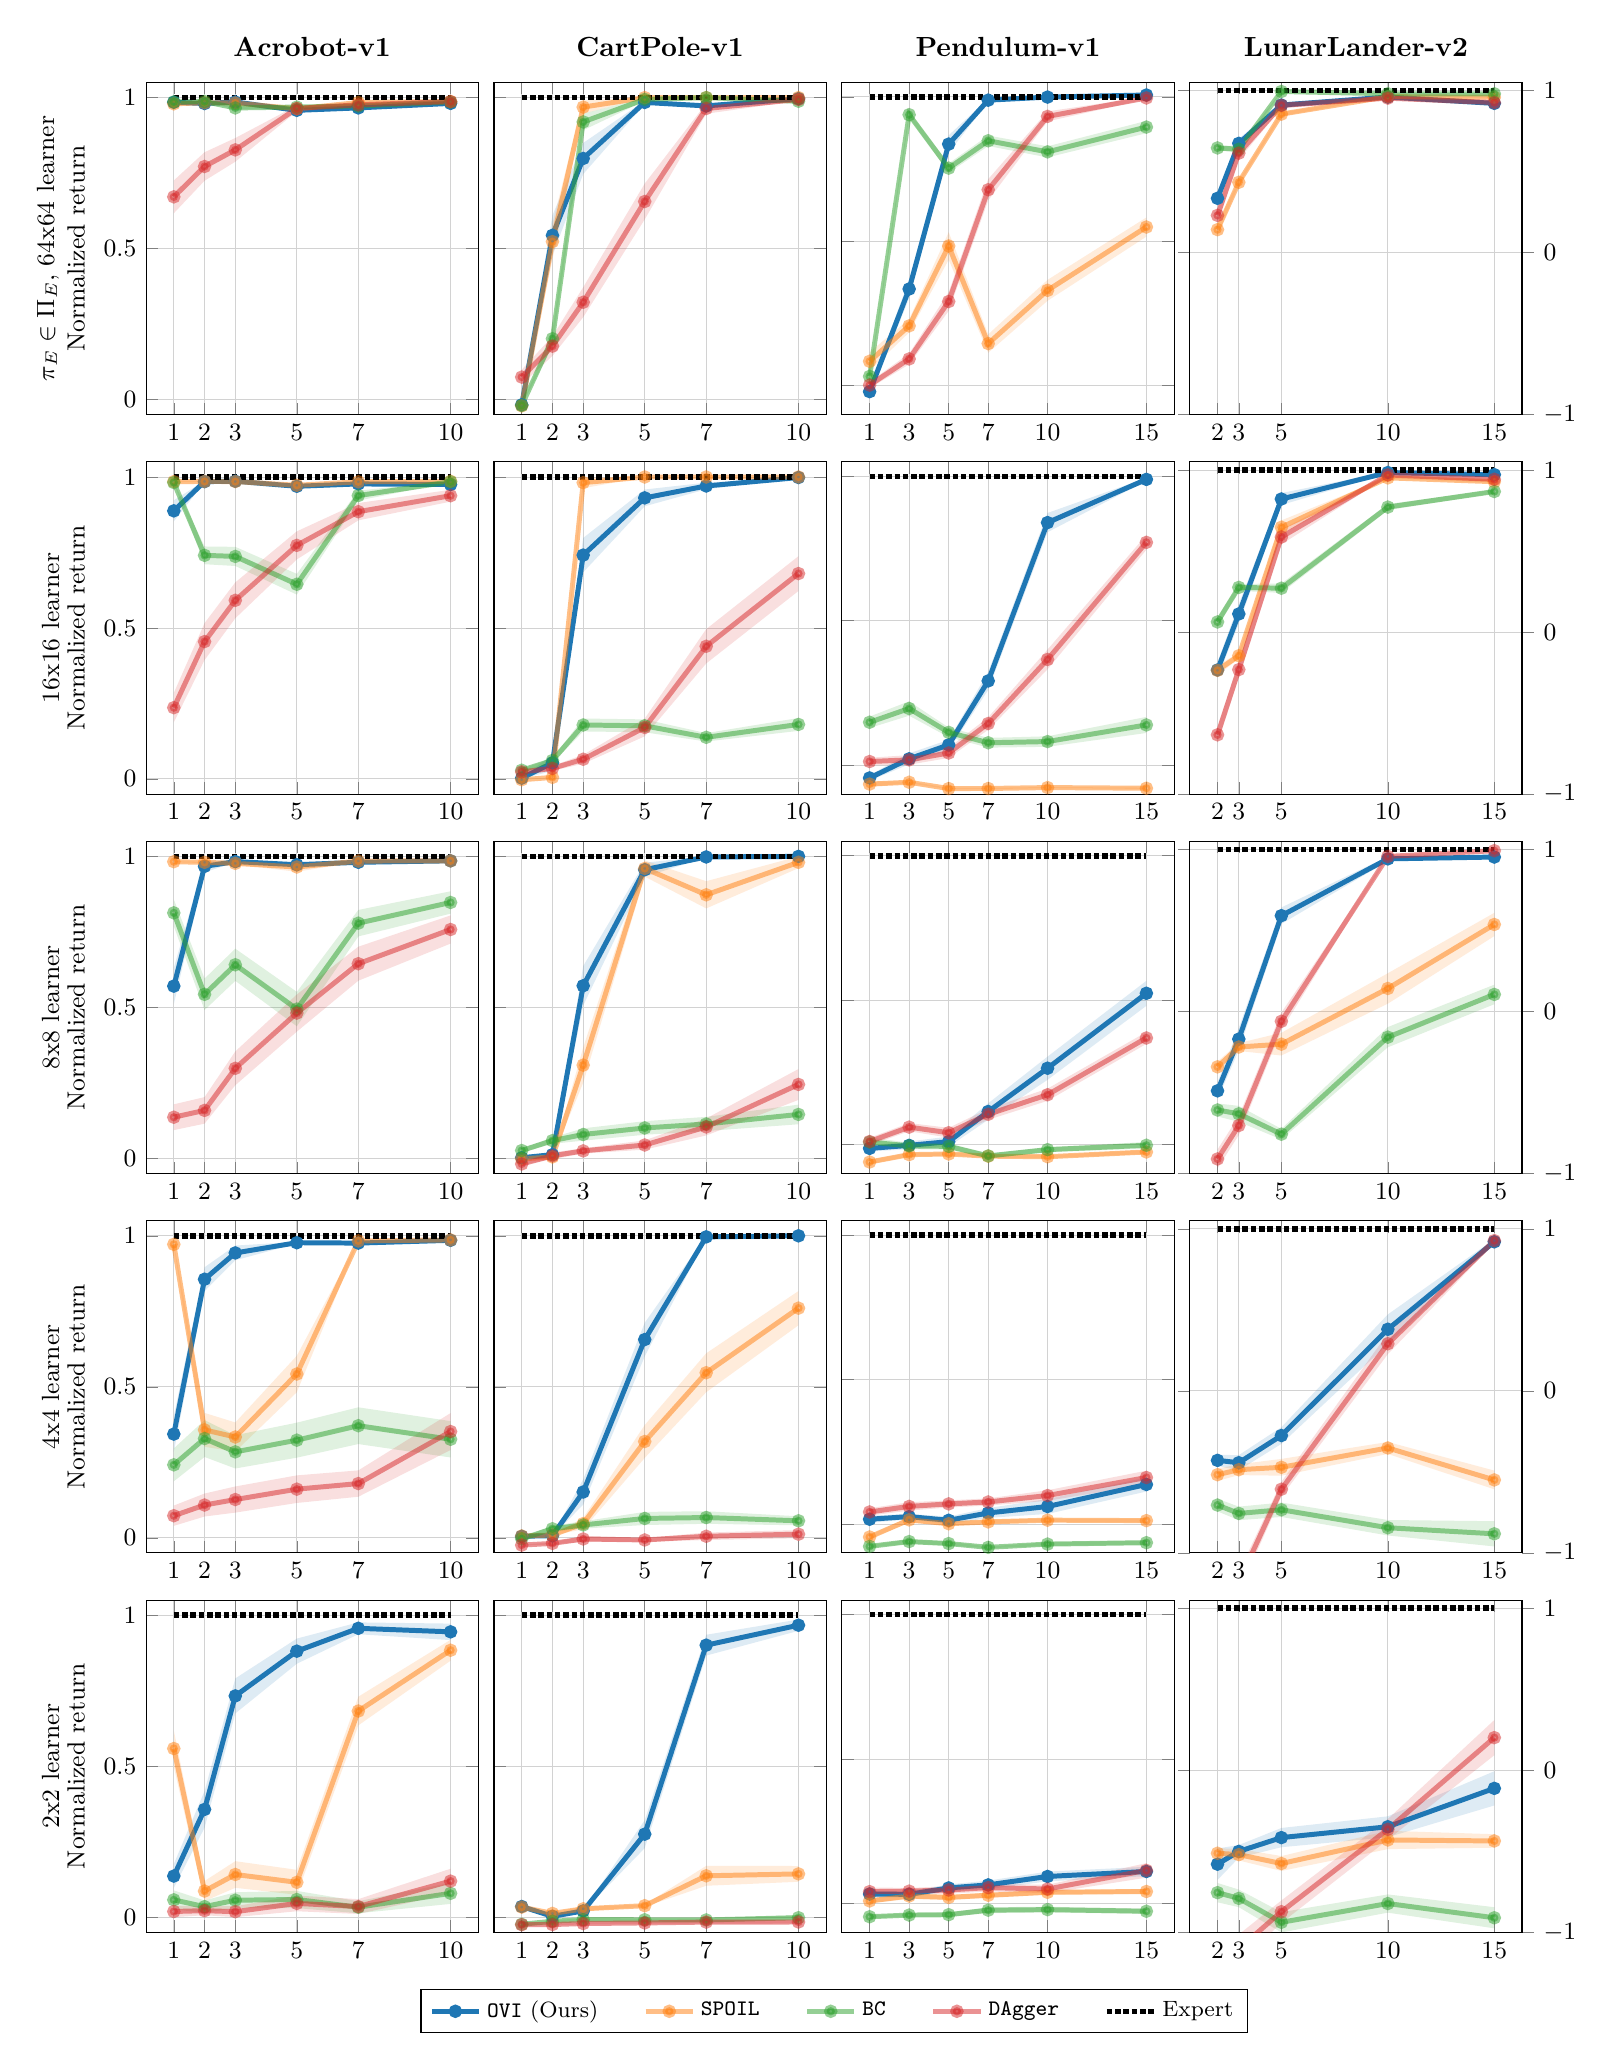
\begin{tikzpicture}
  \begin{groupplot}[
    il plot,
    group style={
      group size=4 by 5,
      horizontal sep=0.2cm,
      vertical sep=0.6cm,
      xlabels at=edge bottom,
      ylabels at=edge left,
    },
  ]
  \nextgroupplot[
    ymin=-0.05,
    ymax=1.05,
    title={Acrobot-v1},
    ylabel={\shortstack[c]{$\pi_E \in \Pi_E$, 64x64 learner\\ \small Normalized return}},
    legend to name=sharedlegend,
    legend columns=-1,
    legend style={font=\footnotesize,/tikz/every even column/.append style={column sep=0.5cm}}
  ]
  % \texttt{OVI} (Ours)
  \addplot[name path=pu0, draw=none, forget plot] coordinates { (1,0.98622) (2,0.98506) (3,0.98797) (5,0.96245) (7,0.97142) (10,0.98352) };
  \addplot[name path=pl0, draw=none, forget plot] coordinates { (1,0.98285) (2,0.97586) (3,0.98282) (5,0.95317) (7,0.96033) (10,0.97811) };
  \addplot[fill=algcol0, fill opacity=0.15, draw=none, forget plot] fill between[of=pu0 and pl0];
  \addplot[algcol0, mark=*, mark size=1.5pt, line width=1.8pt, opacity=1.0] coordinates { (1,0.98453) (2,0.98046) (3,0.98540) (5,0.95781) (7,0.96587) (10,0.98081) };
  \addlegendentry{\texttt{OVI} (Ours)}
  % \texttt{SPOIL}
  \addplot[name path=pu1, draw=none, forget plot] coordinates { (1,0.98164) (2,0.98553) (3,0.98417) (5,0.96732) (7,0.98575) (10,0.98851) };
  \addplot[name path=pl1, draw=none, forget plot] coordinates { (1,0.97723) (2,0.98047) (3,0.98018) (5,0.95854) (7,0.98155) (10,0.98539) };
  \addplot[fill=algcol1, fill opacity=0.15, draw=none, forget plot] fill between[of=pu1 and pl1];
  \addplot[algcol1, mark=*, mark size=1.5pt, line width=1.8pt, opacity=0.5] coordinates { (1,0.97943) (2,0.98300) (3,0.98218) (5,0.96293) (7,0.98365) (10,0.98695) };
  \addlegendentry{\texttt{SPOIL}}
  % \texttt{BC}
  \addplot[name path=pu2, draw=none, forget plot] coordinates { (1,0.98797) (2,0.98822) (3,0.97059) (5,0.97206) (7,0.97636) (10,0.98754) };
  \addplot[name path=pl2, draw=none, forget plot] coordinates { (1,0.98337) (2,0.98565) (3,0.96094) (5,0.96511) (7,0.96801) (10,0.98368) };
  \addplot[fill=algcol2, fill opacity=0.15, draw=none, forget plot] fill between[of=pu2 and pl2];
  \addplot[algcol2, mark=*, mark size=1.5pt, line width=1.8pt, opacity=0.5] coordinates { (1,0.98567) (2,0.98694) (3,0.96576) (5,0.96859) (7,0.97219) (10,0.98561) };
  \addlegendentry{\texttt{BC}}
  % \texttt{DAgger}
  \addplot[name path=pu3, draw=none, forget plot] coordinates { (1,0.72564) (2,0.81900) (3,0.86614) (5,0.97387) (7,0.97946) (10,0.98917) };
  \addplot[name path=pl3, draw=none, forget plot] coordinates { (1,0.61696) (2,0.72463) (3,0.78764) (5,0.95434) (7,0.97238) (10,0.98425) };
  \addplot[fill=algcol3, fill opacity=0.15, draw=none, forget plot] fill between[of=pu3 and pl3];
  \addplot[algcol3, mark=*, mark size=1.5pt, line width=1.8pt, opacity=0.5] coordinates { (1,0.67130) (2,0.77181) (3,0.82689) (5,0.96410) (7,0.97592) (10,0.98671) };
  \addlegendentry{\texttt{DAgger}}
  \addplot[black, densely dotted, line width=2pt, forget plot] coordinates { (1,1.00000) (10,1.00000) };
  \addlegendimage{black, densely dotted, line width=2pt}
  \addlegendentry{Expert}
  \nextgroupplot[
    ymin=-0.05,
    ymax=1.05,
    yticklabels={},
    title={CartPole-v1}
  ]
  % \texttt{OVI} (Ours)
  \addplot[name path=pu4, draw=none, forget plot] coordinates { (1,-0.01625) (2,0.61029) (3,0.84976) (5,0.98941) (7,0.98070) (10,0.99993) };
  \addplot[name path=pl4, draw=none, forget plot] coordinates { (1,-0.01864) (2,0.47736) (3,0.74685) (5,0.97865) (7,0.96414) (10,0.99372) };
  \addplot[fill=algcol0, fill opacity=0.15, draw=none, forget plot] fill between[of=pu4 and pl4];
  \addplot[algcol0, mark=*, mark size=1.5pt, line width=1.8pt, opacity=1.0] coordinates { (1,-0.01744) (2,0.54382) (3,0.79831) (5,0.98403) (7,0.97242) (10,0.99682) };
  % \texttt{SPOIL}
  \addplot[name path=pu5, draw=none, forget plot] coordinates { (1,-0.02034) (2,0.58270) (3,0.99039) (5,1.00000) (7,1.00000) (10,1.00000) };
  \addplot[name path=pl5, draw=none, forget plot] coordinates { (1,-0.02140) (2,0.46352) (3,0.94671) (5,1.00000) (7,1.00000) (10,1.00000) };
  \addplot[fill=algcol1, fill opacity=0.15, draw=none, forget plot] fill between[of=pu5 and pl5];
  \addplot[algcol1, mark=*, mark size=1.5pt, line width=1.8pt, opacity=0.5] coordinates { (1,-0.02087) (2,0.52311) (3,0.96855) (5,1.00000) (7,1.00000) (10,1.00000) };
  % \texttt{BC}
  \addplot[name path=pu6, draw=none, forget plot] coordinates { (1,-0.01919) (2,0.22777) (3,0.94688) (5,0.99931) (7,1.00000) (10,0.99699) };
  \addplot[name path=pl6, draw=none, forget plot] coordinates { (1,-0.02012) (2,0.17529) (3,0.89200) (5,0.98898) (7,1.00000) (10,0.97871) };
  \addplot[fill=algcol2, fill opacity=0.15, draw=none, forget plot] fill between[of=pu6 and pl6];
  \addplot[algcol2, mark=*, mark size=1.5pt, line width=1.8pt, opacity=0.5] coordinates { (1,-0.01965) (2,0.20153) (3,0.91944) (5,0.99415) (7,1.00000) (10,0.98785) };
  % \texttt{DAgger}
  \addplot[name path=pu7, draw=none, forget plot] coordinates { (1,0.09883) (2,0.20932) (3,0.37192) (5,0.71520) (7,0.98104) (10,0.99835) };
  \addplot[name path=pl7, draw=none, forget plot] coordinates { (1,0.04999) (2,0.14460) (3,0.27272) (5,0.59662) (7,0.94660) (10,0.98935) };
  \addplot[fill=algcol3, fill opacity=0.15, draw=none, forget plot] fill between[of=pu7 and pl7];
  \addplot[algcol3, mark=*, mark size=1.5pt, line width=1.8pt, opacity=0.5] coordinates { (1,0.07441) (2,0.17696) (3,0.32232) (5,0.65591) (7,0.96382) (10,0.99385) };
  \addplot[black, densely dotted, line width=2pt, forget plot] coordinates { (1,1.00000) (10,1.00000) };
  \nextgroupplot[
    ymin=-0.1,
    ymax=1.05,
    xtick={1,3,5,7,10,15},
    yticklabels={},
    title={Pendulum-v1}
  ]
  % \texttt{OVI} (Ours)
  \addplot[name path=pu8, draw=none, forget plot] coordinates { (1,-0.00423) (3,0.36702) (5,0.86714) (7,0.99439) (10,1.00332) (15,1.01010) };
  \addplot[name path=pl8, draw=none, forget plot] coordinates { (1,-0.03626) (3,0.30308) (5,0.80637) (7,0.98342) (10,0.99565) (15,1.00317) };
  \addplot[fill=algcol0, fill opacity=0.15, draw=none, forget plot] fill between[of=pu8 and pl8];
  \addplot[algcol0, mark=*, mark size=1.5pt, line width=1.8pt, opacity=1.0] coordinates { (1,-0.02025) (3,0.33505) (5,0.83675) (7,0.98890) (10,0.99949) (15,1.00664) };
  % \texttt{SPOIL}
  \addplot[name path=pu9, draw=none, forget plot] coordinates { (1,0.11654) (3,0.23033) (5,0.53158) (7,0.17801) (10,0.36661) (15,0.58276) };
  \addplot[name path=pl9, draw=none, forget plot] coordinates { (1,0.05308) (3,0.18446) (5,0.43637) (7,0.11430) (10,0.29417) (15,0.51638) };
  \addplot[fill=algcol1, fill opacity=0.15, draw=none, forget plot] fill between[of=pu9 and pl9];
  \addplot[algcol1, mark=*, mark size=1.5pt, line width=1.8pt, opacity=0.5] coordinates { (1,0.08481) (3,0.20739) (5,0.48398) (7,0.14615) (10,0.33039) (15,0.54957) };
  % \texttt{BC}
  \addplot[name path=pu10, draw=none, forget plot] coordinates { (1,0.04610) (3,0.94813) (5,0.76960) (7,0.86642) (10,0.82904) (15,0.91706) };
  \addplot[name path=pl10, draw=none, forget plot] coordinates { (1,0.01868) (3,0.92893) (5,0.73741) (7,0.83011) (10,0.79060) (15,0.87434) };
  \addplot[fill=algcol2, fill opacity=0.15, draw=none, forget plot] fill between[of=pu10 and pl10];
  \addplot[algcol2, mark=*, mark size=1.5pt, line width=1.8pt, opacity=0.5] coordinates { (1,0.03239) (3,0.93853) (5,0.75351) (7,0.84827) (10,0.80982) (15,0.89570) };
  % \texttt{DAgger}
  \addplot[name path=pu11, draw=none, forget plot] coordinates { (1,0.01327) (3,0.11160) (5,0.32441) (7,0.71555) (10,0.94990) (15,1.00064) };
  \addplot[name path=pl11, draw=none, forget plot] coordinates { (1,-0.00855) (3,0.07429) (5,0.25913) (7,0.64193) (10,0.91529) (15,0.99216) };
  \addplot[fill=algcol3, fill opacity=0.15, draw=none, forget plot] fill between[of=pu11 and pl11];
  \addplot[algcol3, mark=*, mark size=1.5pt, line width=1.8pt, opacity=0.5] coordinates { (1,0.00236) (3,0.09294) (5,0.29177) (7,0.67874) (10,0.93259) (15,0.99640) };
  \addplot[black, densely dotted, line width=2pt, forget plot] coordinates { (1,1.00000) (15,1.00000) };
  \nextgroupplot[
    ymin=-1.0,
    ymax=1.05,
    xtick={2,3,5,10,15},
    ytick={-1,0,1},
    yticklabel pos=right,
    ytick align=outside,
    title={LunarLander-v2}
  ]
  % \texttt{OVI} (Ours)
  \addplot[name path=pu12, draw=none, forget plot] coordinates { (2,0.36795) (3,0.70274) (5,0.92716) (10,0.96877) (15,0.93547) };
  \addplot[name path=pl12, draw=none, forget plot] coordinates { (2,0.30272) (3,0.64574) (5,0.89440) (10,0.95172) (15,0.90675) };
  \addplot[fill=algcol0, fill opacity=0.15, draw=none, forget plot] fill between[of=pu12 and pl12];
  \addplot[algcol0, mark=*, mark size=1.5pt, line width=1.8pt, opacity=1.0] coordinates { (2,0.33534) (3,0.67424) (5,0.91078) (10,0.96025) (15,0.92111) };
  % \texttt{SPOIL}
  \addplot[name path=pu13, draw=none, forget plot] coordinates { (2,0.17648) (3,0.44929) (5,0.86696) (10,0.96553) (15,0.96417) };
  \addplot[name path=pl13, draw=none, forget plot] coordinates { (2,0.10716) (3,0.41880) (5,0.84239) (10,0.96014) (15,0.95322) };
  \addplot[fill=algcol1, fill opacity=0.15, draw=none, forget plot] fill between[of=pu13 and pl13];
  \addplot[algcol1, mark=*, mark size=1.5pt, line width=1.8pt, opacity=0.5] coordinates { (2,0.14182) (3,0.43405) (5,0.85468) (10,0.96284) (15,0.95870) };
  % \texttt{BC}
  \addplot[name path=pu14, draw=none, forget plot] coordinates { (2,0.66247) (3,0.65667) (5,0.99638) (10,0.98266) (15,0.98289) };
  \addplot[name path=pl14, draw=none, forget plot] coordinates { (2,0.62989) (3,0.61912) (5,0.99266) (10,0.97824) (15,0.97783) };
  \addplot[fill=algcol2, fill opacity=0.15, draw=none, forget plot] fill between[of=pu14 and pl14];
  \addplot[algcol2, mark=*, mark size=1.5pt, line width=1.8pt, opacity=0.5] coordinates { (2,0.64618) (3,0.63789) (5,0.99452) (10,0.98045) (15,0.98036) };
  % \texttt{DAgger}
  \addplot[name path=pu15, draw=none, forget plot] coordinates { (2,0.28330) (3,0.65355) (5,0.92722) (10,0.96316) (15,0.93718) };
  \addplot[name path=pl15, draw=none, forget plot] coordinates { (2,0.17659) (3,0.57450) (5,0.89053) (10,0.94349) (15,0.91477) };
  \addplot[fill=algcol3, fill opacity=0.15, draw=none, forget plot] fill between[of=pu15 and pl15];
  \addplot[algcol3, mark=*, mark size=1.5pt, line width=1.8pt, opacity=0.5] coordinates { (2,0.22995) (3,0.61402) (5,0.90887) (10,0.95332) (15,0.92597) };
  \addplot[black, densely dotted, line width=2pt, forget plot] coordinates { (2,1.00000) (15,1.00000) };
  \nextgroupplot[
    ymin=-0.05,
    ymax=1.05,
    ylabel={\shortstack[c]{16x16 learner\\ \small Normalized return}}
  ]
  % \texttt{OVI} (Ours)
  \addplot[name path=pu16, draw=none, forget plot] coordinates { (1,0.92278) (2,0.98706) (3,0.98775) (5,0.97317) (7,0.97964) (10,0.97832) };
  \addplot[name path=pl16, draw=none, forget plot] coordinates { (1,0.85309) (2,0.98231) (3,0.98416) (5,0.96535) (7,0.97453) (10,0.97185) };
  \addplot[fill=algcol0, fill opacity=0.15, draw=none, forget plot] fill between[of=pu16 and pl16];
  \addplot[algcol0, mark=*, mark size=1.5pt, line width=1.8pt, opacity=1.0] coordinates { (1,0.88794) (2,0.98469) (3,0.98596) (5,0.96926) (7,0.97708) (10,0.97508) };
  % \texttt{SPOIL}
  \addplot[name path=pu17, draw=none, forget plot] coordinates { (1,0.98624) (2,0.98689) (3,0.98713) (5,0.97603) (7,0.98635) (10,0.98764) };
  \addplot[name path=pl17, draw=none, forget plot] coordinates { (1,0.98303) (2,0.98368) (3,0.98265) (5,0.96906) (7,0.98181) (10,0.98396) };
  \addplot[fill=algcol1, fill opacity=0.15, draw=none, forget plot] fill between[of=pu17 and pl17];
  \addplot[algcol1, mark=*, mark size=1.5pt, line width=1.8pt, opacity=0.5] coordinates { (1,0.98463) (2,0.98529) (3,0.98489) (5,0.97255) (7,0.98408) (10,0.98580) };
  % \texttt{BC}
  \addplot[name path=pu18, draw=none, forget plot] coordinates { (1,0.98429) (2,0.76992) (3,0.76869) (5,0.67922) (7,0.95487) (10,0.98632) };
  \addplot[name path=pl18, draw=none, forget plot] coordinates { (1,0.97913) (2,0.71119) (3,0.70531) (5,0.61054) (7,0.92202) (10,0.98247) };
  \addplot[fill=algcol2, fill opacity=0.15, draw=none, forget plot] fill between[of=pu18 and pl18];
  \addplot[algcol2, mark=*, mark size=1.5pt, line width=1.8pt, opacity=0.5] coordinates { (1,0.98171) (2,0.74056) (3,0.73700) (5,0.64488) (7,0.93844) (10,0.98439) };
  % \texttt{DAgger}
  \addplot[name path=pu19, draw=none, forget plot] coordinates { (1,0.28496) (2,0.51618) (3,0.65098) (5,0.82006) (7,0.91380) (10,0.95769) };
  \addplot[name path=pl19, draw=none, forget plot] coordinates { (1,0.18743) (2,0.39374) (3,0.53210) (5,0.72702) (7,0.85647) (10,0.91845) };
  \addplot[fill=algcol3, fill opacity=0.15, draw=none, forget plot] fill between[of=pu19 and pl19];
  \addplot[algcol3, mark=*, mark size=1.5pt, line width=1.8pt, opacity=0.5] coordinates { (1,0.23619) (2,0.45496) (3,0.59154) (5,0.77354) (7,0.88514) (10,0.93807) };
  \addplot[black, densely dotted, line width=2pt, forget plot] coordinates { (1,1.00000) (10,1.00000) };
  \nextgroupplot[
    ymin=-0.05,
    ymax=1.05,
    yticklabels={}
  ]
  % \texttt{OVI} (Ours)
  \addplot[name path=pu20, draw=none, forget plot] coordinates { (1,0.00498) (2,0.08030) (3,0.79821) (5,0.95859) (7,0.98131) (10,0.99993) };
  \addplot[name path=pl20, draw=none, forget plot] coordinates { (1,0.00078) (2,0.02656) (3,0.68440) (5,0.90311) (7,0.95926) (10,0.99671) };
  \addplot[fill=algcol0, fill opacity=0.15, draw=none, forget plot] fill between[of=pu20 and pl20];
  \addplot[algcol0, mark=*, mark size=1.5pt, line width=1.8pt, opacity=1.0] coordinates { (1,0.00288) (2,0.05343) (3,0.74130) (5,0.93085) (7,0.97028) (10,0.99832) };
  % \texttt{SPOIL}
  \addplot[name path=pu21, draw=none, forget plot] coordinates { (1,-0.00176) (2,0.00596) (3,0.99982) (5,1.00000) (7,1.00000) (10,1.00000) };
  \addplot[name path=pl21, draw=none, forget plot] coordinates { (1,-0.00339) (2,0.00444) (3,0.96283) (5,1.00000) (7,1.00000) (10,1.00000) };
  \addplot[fill=algcol1, fill opacity=0.15, draw=none, forget plot] fill between[of=pu21 and pl21];
  \addplot[algcol1, mark=*, mark size=1.5pt, line width=1.8pt, opacity=0.5] coordinates { (1,-0.00258) (2,0.00520) (3,0.98133) (5,1.00000) (7,1.00000) (10,1.00000) };
  % \texttt{BC}
  \addplot[name path=pu22, draw=none, forget plot] coordinates { (1,0.03300) (2,0.06938) (3,0.20020) (5,0.19730) (7,0.15183) (10,0.20190) };
  \addplot[name path=pl22, draw=none, forget plot] coordinates { (1,0.02480) (2,0.05303) (3,0.15738) (5,0.15464) (7,0.12400) (10,0.15927) };
  \addplot[fill=algcol2, fill opacity=0.15, draw=none, forget plot] fill between[of=pu22 and pl22];
  \addplot[algcol2, mark=*, mark size=1.5pt, line width=1.8pt, opacity=0.5] coordinates { (1,0.02890) (2,0.06121) (3,0.17879) (5,0.17597) (7,0.13792) (10,0.18058) };
  % \texttt{DAgger}
  \addplot[name path=pu23, draw=none, forget plot] coordinates { (1,0.03392) (2,0.04354) (3,0.08002) (5,0.20007) (7,0.49624) (10,0.73789) };
  \addplot[name path=pl23, draw=none, forget plot] coordinates { (1,0.01266) (2,0.02669) (3,0.05070) (5,0.14118) (7,0.38258) (10,0.62259) };
  \addplot[fill=algcol3, fill opacity=0.15, draw=none, forget plot] fill between[of=pu23 and pl23];
  \addplot[algcol3, mark=*, mark size=1.5pt, line width=1.8pt, opacity=0.5] coordinates { (1,0.02329) (2,0.03512) (3,0.06536) (5,0.17062) (7,0.43941) (10,0.68024) };
  \addplot[black, densely dotted, line width=2pt, forget plot] coordinates { (1,1.00000) (10,1.00000) };
  \nextgroupplot[
    ymin=-0.1,
    ymax=1.05,
    xtick={1,3,5,7,10,15},
    yticklabels={}
  ]
  % \texttt{OVI} (Ours)
  \addplot[name path=pu24, draw=none, forget plot] coordinates { (1,-0.03466) (3,0.04085) (5,0.08795) (7,0.32295) (10,0.87318) (15,0.99444) };
  \addplot[name path=pl24, draw=none, forget plot] coordinates { (1,-0.05378) (3,0.00315) (5,0.05282) (7,0.26061) (10,0.80663) (15,0.98447) };
  \addplot[fill=algcol0, fill opacity=0.15, draw=none, forget plot] fill between[of=pu24 and pl24];
  \addplot[algcol0, mark=*, mark size=1.5pt, line width=1.8pt, opacity=1.0] coordinates { (1,-0.04422) (3,0.02200) (5,0.07038) (7,0.29178) (10,0.83991) (15,0.98945) };
  % \texttt{SPOIL}
  \addplot[name path=pu25, draw=none, forget plot] coordinates { (1,-0.05579) (3,-0.05576) (5,-0.07865) (7,-0.07827) (10,-0.07551) (15,-0.07745) };
  \addplot[name path=pl25, draw=none, forget plot] coordinates { (1,-0.07520) (3,-0.06246) (5,-0.08311) (7,-0.08305) (10,-0.07955) (15,-0.08216) };
  \addplot[fill=algcol1, fill opacity=0.15, draw=none, forget plot] fill between[of=pu25 and pl25];
  \addplot[algcol1, mark=*, mark size=1.5pt, line width=1.8pt, opacity=0.5] coordinates { (1,-0.06550) (3,-0.05911) (5,-0.08088) (7,-0.08066) (10,-0.07753) (15,-0.07980) };
  % \texttt{BC}
  \addplot[name path=pu26, draw=none, forget plot] coordinates { (1,0.16833) (3,0.22105) (5,0.13016) (7,0.09444) (10,0.10002) (15,0.16713) };
  \addplot[name path=pl26, draw=none, forget plot] coordinates { (1,0.12874) (3,0.17132) (5,0.09695) (7,0.06077) (10,0.06350) (15,0.11153) };
  \addplot[fill=algcol2, fill opacity=0.15, draw=none, forget plot] fill between[of=pu26 and pl26];
  \addplot[algcol2, mark=*, mark size=1.5pt, line width=1.8pt, opacity=0.5] coordinates { (1,0.14854) (3,0.19619) (5,0.11356) (7,0.07760) (10,0.08176) (15,0.13933) };
  % \texttt{DAgger}
  \addplot[name path=pu27, draw=none, forget plot] coordinates { (1,0.02584) (3,0.03487) (5,0.05946) (7,0.16592) (10,0.40032) (15,0.79698) };
  \addplot[name path=pl27, draw=none, forget plot] coordinates { (1,-0.00046) (3,0.00180) (5,0.02496) (7,0.12255) (10,0.33183) (15,0.74585) };
  \addplot[fill=algcol3, fill opacity=0.15, draw=none, forget plot] fill between[of=pu27 and pl27];
  \addplot[algcol3, mark=*, mark size=1.5pt, line width=1.8pt, opacity=0.5] coordinates { (1,0.01269) (3,0.01833) (5,0.04221) (7,0.14423) (10,0.36608) (15,0.77141) };
  \addplot[black, densely dotted, line width=2pt, forget plot] coordinates { (1,1.00000) (15,1.00000) };
  \nextgroupplot[
    ymin=-1.0,
    ymax=1.05,
    xtick={2,3,5,10,15},
    ytick={-1,0,1},
    yticklabel pos=right,
    ytick align=outside
  ]
  % \texttt{OVI} (Ours)
  \addplot[name path=pu28, draw=none, forget plot] coordinates { (2,-0.18520) (3,0.17186) (5,0.85768) (10,0.98913) (15,0.97765) };
  \addplot[name path=pl28, draw=none, forget plot] coordinates { (2,-0.28326) (3,0.05159) (5,0.78421) (10,0.97949) (15,0.96515) };
  \addplot[fill=algcol0, fill opacity=0.15, draw=none, forget plot] fill between[of=pu28 and pl28];
  \addplot[algcol0, mark=*, mark size=1.5pt, line width=1.8pt, opacity=1.0] coordinates { (2,-0.23423) (3,0.11172) (5,0.82095) (10,0.98431) (15,0.97140) };
  % \texttt{SPOIL}
  \addplot[name path=pu29, draw=none, forget plot] coordinates { (2,-0.20690) (3,-0.12744) (5,0.68889) (10,0.95582) (15,0.93525) };
  \addplot[name path=pl29, draw=none, forget plot] coordinates { (2,-0.26597) (3,-0.16555) (5,0.60470) (10,0.94718) (15,0.92041) };
  \addplot[fill=algcol1, fill opacity=0.15, draw=none, forget plot] fill between[of=pu29 and pl29];
  \addplot[algcol1, mark=*, mark size=1.5pt, line width=1.8pt, opacity=0.5] coordinates { (2,-0.23643) (3,-0.14649) (5,0.64680) (10,0.95150) (15,0.92783) };
  % \texttt{BC}
  \addplot[name path=pu30, draw=none, forget plot] coordinates { (2,0.09197) (3,0.29694) (5,0.29934) (10,0.79013) (15,0.87900) };
  \addplot[name path=pl30, draw=none, forget plot] coordinates { (2,0.03271) (3,0.25417) (5,0.24163) (10,0.75216) (15,0.85558) };
  \addplot[fill=algcol2, fill opacity=0.15, draw=none, forget plot] fill between[of=pu30 and pl30];
  \addplot[algcol2, mark=*, mark size=1.5pt, line width=1.8pt, opacity=0.5] coordinates { (2,0.06234) (3,0.27555) (5,0.27048) (10,0.77115) (15,0.86729) };
  % \texttt{DAgger}
  \addplot[name path=pu31, draw=none, forget plot] coordinates { (2,-0.58236) (3,-0.18215) (5,0.63189) (10,0.97820) (15,0.95731) };
  \addplot[name path=pl31, draw=none, forget plot] coordinates { (2,-0.68630) (3,-0.28157) (5,0.54107) (10,0.96081) (15,0.92778) };
  \addplot[fill=algcol3, fill opacity=0.15, draw=none, forget plot] fill between[of=pu31 and pl31];
  \addplot[algcol3, mark=*, mark size=1.5pt, line width=1.8pt, opacity=0.5] coordinates { (2,-0.63433) (3,-0.23186) (5,0.58648) (10,0.96951) (15,0.94255) };
  \addplot[black, densely dotted, line width=2pt, forget plot] coordinates { (2,1.00000) (15,1.00000) };
  \nextgroupplot[
    ymin=-0.05,
    ymax=1.05,
    ylabel={\shortstack[c]{8x8 learner\\ \small Normalized return}}
  ]
  % \texttt{OVI} (Ours)
  \addplot[name path=pu32, draw=none, forget plot] coordinates { (1,0.63045) (2,0.98666) (3,0.98498) (5,0.97557) (7,0.98288) (10,0.98856) };
  \addplot[name path=pl32, draw=none, forget plot] coordinates { (1,0.51048) (2,0.94743) (3,0.98081) (5,0.96927) (7,0.97821) (10,0.98215) };
  \addplot[fill=algcol0, fill opacity=0.15, draw=none, forget plot] fill between[of=pu32 and pl32];
  \addplot[algcol0, mark=*, mark size=1.5pt, line width=1.8pt, opacity=1.0] coordinates { (1,0.57047) (2,0.96704) (3,0.98290) (5,0.97242) (7,0.98054) (10,0.98536) };
  % \texttt{SPOIL}
  \addplot[name path=pu33, draw=none, forget plot] coordinates { (1,0.98446) (2,0.98252) (3,0.98068) (5,0.98071) (7,0.98678) (10,0.98701) };
  \addplot[name path=pl33, draw=none, forget plot] coordinates { (1,0.98057) (2,0.97798) (3,0.97318) (5,0.94911) (7,0.98237) (10,0.98364) };
  \addplot[fill=algcol1, fill opacity=0.15, draw=none, forget plot] fill between[of=pu33 and pl33];
  \addplot[algcol1, mark=*, mark size=1.5pt, line width=1.8pt, opacity=0.5] coordinates { (1,0.98252) (2,0.98025) (3,0.97693) (5,0.96491) (7,0.98457) (10,0.98533) };
  % \texttt{BC}
  \addplot[name path=pu34, draw=none, forget plot] coordinates { (1,0.85747) (2,0.59542) (3,0.69441) (5,0.55141) (7,0.82269) (10,0.88449) };
  \addplot[name path=pl34, draw=none, forget plot] coordinates { (1,0.76862) (2,0.49105) (3,0.58794) (5,0.43748) (7,0.73509) (10,0.81051) };
  \addplot[fill=algcol2, fill opacity=0.15, draw=none, forget plot] fill between[of=pu34 and pl34];
  \addplot[algcol2, mark=*, mark size=1.5pt, line width=1.8pt, opacity=0.5] coordinates { (1,0.81304) (2,0.54323) (3,0.64117) (5,0.49445) (7,0.77889) (10,0.84750) };
  % \texttt{DAgger}
  \addplot[name path=pu35, draw=none, forget plot] coordinates { (1,0.17897) (2,0.20287) (3,0.35421) (5,0.54273) (7,0.70100) (10,0.80457) };
  \addplot[name path=pl35, draw=none, forget plot] coordinates { (1,0.09360) (2,0.11500) (3,0.24221) (5,0.41969) (7,0.58836) (10,0.71126) };
  \addplot[fill=algcol3, fill opacity=0.15, draw=none, forget plot] fill between[of=pu35 and pl35];
  \addplot[algcol3, mark=*, mark size=1.5pt, line width=1.8pt, opacity=0.5] coordinates { (1,0.13628) (2,0.15894) (3,0.29821) (5,0.48121) (7,0.64468) (10,0.75791) };
  \addplot[black, densely dotted, line width=2pt, forget plot] coordinates { (1,1.00000) (10,1.00000) };
  \nextgroupplot[
    ymin=-0.05,
    ymax=1.05,
    yticklabels={}
  ]
  % \texttt{OVI} (Ours)
  \addplot[name path=pu36, draw=none, forget plot] coordinates { (1,0.00315) (2,0.01570) (3,0.63709) (5,0.97924) (7,0.99998) (10,1.00000) };
  \addplot[name path=pl36, draw=none, forget plot] coordinates { (1,0.00082) (2,0.00909) (3,0.50622) (5,0.93271) (7,0.99634) (10,1.00000) };
  \addplot[fill=algcol0, fill opacity=0.15, draw=none, forget plot] fill between[of=pu36 and pl36];
  \addplot[algcol0, mark=*, mark size=1.5pt, line width=1.8pt, opacity=1.0] coordinates { (1,0.00199) (2,0.01240) (3,0.57165) (5,0.95597) (7,0.99816) (10,1.00000) };
  % \texttt{SPOIL}
  \addplot[name path=pu37, draw=none, forget plot] coordinates { (1,-0.00111) (2,0.00541) (3,0.36736) (5,0.98682) (7,0.91793) (10,0.99980) };
  \addplot[name path=pl37, draw=none, forget plot] coordinates { (1,-0.00218) (2,0.00396) (3,0.25032) (5,0.93317) (7,0.82778) (10,0.96110) };
  \addplot[fill=algcol1, fill opacity=0.15, draw=none, forget plot] fill between[of=pu37 and pl37];
  \addplot[algcol1, mark=*, mark size=1.5pt, line width=1.8pt, opacity=0.5] coordinates { (1,-0.00165) (2,0.00468) (3,0.30884) (5,0.96000) (7,0.87286) (10,0.98045) };
  % \texttt{BC}
  \addplot[name path=pu38, draw=none, forget plot] coordinates { (1,0.03239) (2,0.06925) (3,0.09945) (5,0.12320) (7,0.13739) (10,0.17798) };
  \addplot[name path=pl38, draw=none, forget plot] coordinates { (1,0.01961) (2,0.04829) (3,0.05874) (5,0.07822) (7,0.09046) (10,0.11298) };
  \addplot[fill=algcol2, fill opacity=0.15, draw=none, forget plot] fill between[of=pu38 and pl38];
  \addplot[algcol2, mark=*, mark size=1.5pt, line width=1.8pt, opacity=0.5] coordinates { (1,0.02600) (2,0.05877) (3,0.07910) (5,0.10071) (7,0.11392) (10,0.14548) };
  % \texttt{DAgger}
  \addplot[name path=pu39, draw=none, forget plot] coordinates { (1,-0.01534) (2,0.01971) (3,0.03367) (5,0.05959) (7,0.13222) (10,0.29593) };
  \addplot[name path=pl39, draw=none, forget plot] coordinates { (1,-0.02155) (2,-0.00280) (3,0.01594) (5,0.02893) (7,0.07599) (10,0.19367) };
  \addplot[fill=algcol3, fill opacity=0.15, draw=none, forget plot] fill between[of=pu39 and pl39];
  \addplot[algcol3, mark=*, mark size=1.5pt, line width=1.8pt, opacity=0.5] coordinates { (1,-0.01844) (2,0.00845) (3,0.02481) (5,0.04426) (7,0.10410) (10,0.24480) };
  \addplot[black, densely dotted, line width=2pt, forget plot] coordinates { (1,1.00000) (10,1.00000) };
  \nextgroupplot[
    ymin=-0.1,
    ymax=1.05,
    xtick={1,3,5,7,10,15},
    yticklabels={}
  ]
  % \texttt{OVI} (Ours)
  \addplot[name path=pu40, draw=none, forget plot] coordinates { (1,-0.00273) (3,0.01083) (5,0.02776) (7,0.14306) (10,0.30452) (15,0.56709) };
  \addplot[name path=pl40, draw=none, forget plot] coordinates { (1,-0.02361) (3,-0.01617) (5,-0.00706) (7,0.08591) (10,0.22432) (15,0.48056) };
  \addplot[fill=algcol0, fill opacity=0.15, draw=none, forget plot] fill between[of=pu40 and pl40];
  \addplot[algcol0, mark=*, mark size=1.5pt, line width=1.8pt, opacity=1.0] coordinates { (1,-0.01317) (3,-0.00267) (5,0.01035) (7,0.11448) (10,0.26442) (15,0.52383) };
  % \texttt{SPOIL}
  \addplot[name path=pu41, draw=none, forget plot] coordinates { (1,-0.05260) (3,-0.02822) (5,-0.02712) (7,-0.03439) (10,-0.03673) (15,-0.01851) };
  \addplot[name path=pl41, draw=none, forget plot] coordinates { (1,-0.06809) (3,-0.04143) (5,-0.03793) (7,-0.04575) (10,-0.04749) (15,-0.03253) };
  \addplot[fill=algcol1, fill opacity=0.15, draw=none, forget plot] fill between[of=pu41 and pl41];
  \addplot[algcol1, mark=*, mark size=1.5pt, line width=1.8pt, opacity=0.5] coordinates { (1,-0.06034) (3,-0.03483) (5,-0.03252) (7,-0.04007) (10,-0.04211) (15,-0.02552) };
  % \texttt{BC}
  \addplot[name path=pu42, draw=none, forget plot] coordinates { (1,0.02426) (3,0.00669) (5,0.00466) (7,-0.03121) (10,-0.00878) (15,0.00899) };
  \addplot[name path=pl42, draw=none, forget plot] coordinates { (1,-0.00686) (3,-0.01574) (5,-0.01704) (7,-0.04728) (10,-0.02615) (15,-0.01374) };
  \addplot[fill=algcol2, fill opacity=0.15, draw=none, forget plot] fill between[of=pu42 and pl42];
  \addplot[algcol2, mark=*, mark size=1.5pt, line width=1.8pt, opacity=0.5] coordinates { (1,0.00870) (3,-0.00452) (5,-0.00619) (7,-0.03925) (10,-0.01747) (15,-0.00237) };
  % \texttt{DAgger}
  \addplot[name path=pu43, draw=none, forget plot] coordinates { (1,0.02336) (3,0.07455) (5,0.05803) (7,0.12380) (10,0.19376) (15,0.38965) };
  \addplot[name path=pl43, draw=none, forget plot] coordinates { (1,-0.00203) (3,0.04628) (5,0.02401) (7,0.08595) (10,0.15146) (15,0.34863) };
  \addplot[fill=algcol3, fill opacity=0.15, draw=none, forget plot] fill between[of=pu43 and pl43];
  \addplot[algcol3, mark=*, mark size=1.5pt, line width=1.8pt, opacity=0.5] coordinates { (1,0.01066) (3,0.06042) (5,0.04102) (7,0.10488) (10,0.17261) (15,0.36914) };
  \addplot[black, densely dotted, line width=2pt, forget plot] coordinates { (1,1.00000) (15,1.00000) };
  \nextgroupplot[
    ymin=-1.0,
    ymax=1.05,
    xtick={2,3,5,10,15},
    ytick={-1,0,1},
    yticklabel pos=right,
    ytick align=outside
  ]
  % \texttt{OVI} (Ours)
  \addplot[name path=pu44, draw=none, forget plot] coordinates { (2,-0.43766) (3,-0.10216) (5,0.64189) (10,0.95589) (15,0.96196) };
  \addplot[name path=pl44, draw=none, forget plot] coordinates { (2,-0.54198) (3,-0.23925) (5,0.54030) (10,0.92760) (15,0.94394) };
  \addplot[fill=algcol0, fill opacity=0.15, draw=none, forget plot] fill between[of=pu44 and pl44];
  \addplot[algcol0, mark=*, mark size=1.5pt, line width=1.8pt, opacity=1.0] coordinates { (2,-0.48982) (3,-0.17071) (5,0.59110) (10,0.94174) (15,0.95295) };
  % \texttt{SPOIL}
  \addplot[name path=pu45, draw=none, forget plot] coordinates { (2,-0.30883) (3,-0.19511) (5,-0.13189) (10,0.23576) (15,0.60850) };
  \addplot[name path=pl45, draw=none, forget plot] coordinates { (2,-0.37491) (3,-0.24397) (5,-0.27198) (10,0.04799) (15,0.46512) };
  \addplot[fill=algcol1, fill opacity=0.15, draw=none, forget plot] fill between[of=pu45 and pl45];
  \addplot[algcol1, mark=*, mark size=1.5pt, line width=1.8pt, opacity=0.5] coordinates { (2,-0.34187) (3,-0.21954) (5,-0.20193) (10,0.14187) (15,0.53681) };
  % \texttt{BC}
  \addplot[name path=pu46, draw=none, forget plot] coordinates { (2,-0.56794) (3,-0.58280) (5,-0.72468) (10,-0.09647) (15,0.16549) };
  \addplot[name path=pl46, draw=none, forget plot] coordinates { (2,-0.64839) (3,-0.68092) (5,-0.79031) (10,-0.22114) (15,0.04456) };
  \addplot[fill=algcol2, fill opacity=0.15, draw=none, forget plot] fill between[of=pu46 and pl46];
  \addplot[algcol2, mark=*, mark size=1.5pt, line width=1.8pt, opacity=0.5] coordinates { (2,-0.60817) (3,-0.63186) (5,-0.75749) (10,-0.15880) (15,0.10502) };
  % \texttt{DAgger}
  \addplot[name path=pu47, draw=none, forget plot] coordinates { (2,-0.85176) (3,-0.64556) (5,-0.00683) (10,0.96519) (15,0.99558) };
  \addplot[name path=pl47, draw=none, forget plot] coordinates { (2,-0.96888) (3,-0.76279) (5,-0.11454) (10,0.94833) (15,0.98882) };
  \addplot[fill=algcol3, fill opacity=0.15, draw=none, forget plot] fill between[of=pu47 and pl47];
  \addplot[algcol3, mark=*, mark size=1.5pt, line width=1.8pt, opacity=0.5] coordinates { (2,-0.91032) (3,-0.70417) (5,-0.06069) (10,0.95676) (15,0.99220) };
  \addplot[black, densely dotted, line width=2pt, forget plot] coordinates { (2,1.00000) (15,1.00000) };
  \nextgroupplot[
    ymin=-0.05,
    ymax=1.05,
    ylabel={\shortstack[c]{4x4 learner\\ \small Normalized return}}
  ]
  % \texttt{OVI} (Ours)
  \addplot[name path=pu48, draw=none, forget plot] coordinates { (1,0.40246) (2,0.89580) (3,0.96772) (5,0.97983) (7,0.97840) (10,0.98688) };
  \addplot[name path=pl48, draw=none, forget plot] coordinates { (1,0.28435) (2,0.81658) (3,0.91897) (5,0.97448) (7,0.97340) (10,0.98343) };
  \addplot[fill=algcol0, fill opacity=0.15, draw=none, forget plot] fill between[of=pu48 and pl48];
  \addplot[algcol0, mark=*, mark size=1.5pt, line width=1.8pt, opacity=1.0] coordinates { (1,0.34341) (2,0.85619) (3,0.94334) (5,0.97716) (7,0.97590) (10,0.98515) };
  % \texttt{SPOIL}
  \addplot[name path=pu49, draw=none, forget plot] coordinates { (1,0.97675) (2,0.41349) (3,0.38192) (5,0.60275) (7,0.98512) (10,0.98779) };
  \addplot[name path=pl49, draw=none, forget plot] coordinates { (1,0.96673) (2,0.30130) (3,0.28559) (5,0.48203) (7,0.98108) (10,0.98508) };
  \addplot[fill=algcol1, fill opacity=0.15, draw=none, forget plot] fill between[of=pu49 and pl49];
  \addplot[algcol1, mark=*, mark size=1.5pt, line width=1.8pt, opacity=0.5] coordinates { (1,0.97174) (2,0.35739) (3,0.33375) (5,0.54239) (7,0.98310) (10,0.98643) };
  % \texttt{BC}
  \addplot[name path=pu50, draw=none, forget plot] coordinates { (1,0.29623) (2,0.38952) (3,0.33954) (5,0.38122) (7,0.43200) (10,0.38635) };
  \addplot[name path=pl50, draw=none, forget plot] coordinates { (1,0.18702) (2,0.26761) (3,0.22945) (5,0.26534) (7,0.31036) (10,0.26600) };
  \addplot[fill=algcol2, fill opacity=0.15, draw=none, forget plot] fill between[of=pu50 and pl50];
  \addplot[algcol2, mark=*, mark size=1.5pt, line width=1.8pt, opacity=0.5] coordinates { (1,0.24163) (2,0.32856) (3,0.28449) (5,0.32328) (7,0.37118) (10,0.32618) };
  % \texttt{DAgger}
  \addplot[name path=pu51, draw=none, forget plot] coordinates { (1,0.10666) (2,0.14652) (3,0.16993) (5,0.20667) (7,0.22320) (10,0.41298) };
  \addplot[name path=pl51, draw=none, forget plot] coordinates { (1,0.03949) (2,0.07043) (3,0.08333) (5,0.11533) (7,0.13594) (10,0.29079) };
  \addplot[fill=algcol3, fill opacity=0.15, draw=none, forget plot] fill between[of=pu51 and pl51];
  \addplot[algcol3, mark=*, mark size=1.5pt, line width=1.8pt, opacity=0.5] coordinates { (1,0.07308) (2,0.10847) (3,0.12663) (5,0.16100) (7,0.17957) (10,0.35188) };
  \addplot[black, densely dotted, line width=2pt, forget plot] coordinates { (1,1.00000) (10,1.00000) };
  \nextgroupplot[
    ymin=-0.05,
    ymax=1.05,
    yticklabels={}
  ]
  % \texttt{OVI} (Ours)
  \addplot[name path=pu52, draw=none, forget plot] coordinates { (1,0.00640) (2,0.00832) (3,0.19354) (5,0.71212) (7,0.99997) (10,1.00000) };
  \addplot[name path=pl52, draw=none, forget plot] coordinates { (1,0.00337) (2,0.00610) (3,0.10977) (5,0.60062) (7,0.99313) (10,1.00000) };
  \addplot[fill=algcol0, fill opacity=0.15, draw=none, forget plot] fill between[of=pu52 and pl52];
  \addplot[algcol0, mark=*, mark size=1.5pt, line width=1.8pt, opacity=1.0] coordinates { (1,0.00488) (2,0.00721) (3,0.15166) (5,0.65637) (7,0.99655) (10,1.00000) };
  % \texttt{SPOIL}
  \addplot[name path=pu53, draw=none, forget plot] coordinates { (1,0.00731) (2,0.01018) (3,0.06571) (5,0.37325) (7,0.61099) (10,0.81723) };
  \addplot[name path=pl53, draw=none, forget plot] coordinates { (1,0.00462) (2,0.00818) (3,0.02808) (5,0.26446) (7,0.48221) (10,0.70379) };
  \addplot[fill=algcol1, fill opacity=0.15, draw=none, forget plot] fill between[of=pu53 and pl53];
  \addplot[algcol1, mark=*, mark size=1.5pt, line width=1.8pt, opacity=0.5] coordinates { (1,0.00596) (2,0.00918) (3,0.04689) (5,0.31885) (7,0.54660) (10,0.76051) };
  % \texttt{BC}
  \addplot[name path=pu54, draw=none, forget plot] coordinates { (1,0.00140) (2,0.03982) (3,0.05442) (5,0.08576) (7,0.08790) (10,0.07121) };
  \addplot[name path=pl54, draw=none, forget plot] coordinates { (1,-0.00817) (2,0.01981) (3,0.03053) (5,0.04225) (7,0.04630) (10,0.04126) };
  \addplot[fill=algcol2, fill opacity=0.15, draw=none, forget plot] fill between[of=pu54 and pl54];
  \addplot[algcol2, mark=*, mark size=1.5pt, line width=1.8pt, opacity=0.5] coordinates { (1,-0.00339) (2,0.02982) (3,0.04247) (5,0.06401) (7,0.06710) (10,0.05623) };
  % \texttt{DAgger}
  \addplot[name path=pu55, draw=none, forget plot] coordinates { (1,-0.02260) (2,-0.01501) (3,0.00628) (5,-0.00097) (7,0.01744) (10,0.02548) };
  \addplot[name path=pl55, draw=none, forget plot] coordinates { (1,-0.02589) (2,-0.02215) (3,-0.01403) (5,-0.01352) (7,-0.00741) (10,-0.00161) };
  \addplot[fill=algcol3, fill opacity=0.15, draw=none, forget plot] fill between[of=pu55 and pl55];
  \addplot[algcol3, mark=*, mark size=1.5pt, line width=1.8pt, opacity=0.5] coordinates { (1,-0.02424) (2,-0.01858) (3,-0.00387) (5,-0.00725) (7,0.00501) (10,0.01194) };
  \addplot[black, densely dotted, line width=2pt, forget plot] coordinates { (1,1.00000) (10,1.00000) };
  \nextgroupplot[
    ymin=-0.1,
    ymax=1.05,
    xtick={1,3,5,7,10,15},
    yticklabels={}
  ]
  % \texttt{OVI} (Ours)
  \addplot[name path=pu56, draw=none, forget plot] coordinates { (1,0.02896) (3,0.03485) (5,0.02579) (7,0.05513) (10,0.08631) (15,0.16119) };
  \addplot[name path=pl56, draw=none, forget plot] coordinates { (1,0.00402) (3,0.01645) (5,-0.00009) (7,0.02123) (10,0.03485) (15,0.11247) };
  \addplot[fill=algcol0, fill opacity=0.15, draw=none, forget plot] fill between[of=pu56 and pl56];
  \addplot[algcol0, mark=*, mark size=1.5pt, line width=1.8pt, opacity=1.0] coordinates { (1,0.01649) (3,0.02565) (5,0.01285) (7,0.03818) (10,0.06058) (15,0.13683) };
  % \texttt{SPOIL}
  \addplot[name path=pu57, draw=none, forget plot] coordinates { (1,-0.03865) (3,0.02487) (5,0.00670) (7,0.01472) (10,0.01887) (15,0.01851) };
  \addplot[name path=pl57, draw=none, forget plot] coordinates { (1,-0.05130) (3,0.00380) (5,-0.00486) (7,-0.00005) (10,0.00761) (15,0.00496) };
  \addplot[fill=algcol1, fill opacity=0.15, draw=none, forget plot] fill between[of=pu57 and pl57];
  \addplot[algcol1, mark=*, mark size=1.5pt, line width=1.8pt, opacity=0.5] coordinates { (1,-0.04498) (3,0.01434) (5,0.00092) (7,0.00733) (10,0.01324) (15,0.01174) };
  % \texttt{BC}
  \addplot[name path=pu58, draw=none, forget plot] coordinates { (1,-0.07297) (3,-0.05277) (5,-0.06113) (7,-0.07766) (10,-0.06312) (15,-0.05671) };
  \addplot[name path=pl58, draw=none, forget plot] coordinates { (1,-0.08196) (3,-0.06888) (5,-0.07437) (7,-0.08400) (10,-0.07598) (15,-0.07269) };
  \addplot[fill=algcol2, fill opacity=0.15, draw=none, forget plot] fill between[of=pu58 and pl58];
  \addplot[algcol2, mark=*, mark size=1.5pt, line width=1.8pt, opacity=0.5] coordinates { (1,-0.07746) (3,-0.06082) (5,-0.06775) (7,-0.08083) (10,-0.06955) (15,-0.06470) };
  % \texttt{DAgger}
  \addplot[name path=pu59, draw=none, forget plot] coordinates { (1,0.05442) (3,0.07546) (5,0.08186) (7,0.08860) (10,0.11693) (15,0.18457) };
  \addplot[name path=pl59, draw=none, forget plot] coordinates { (1,0.02895) (3,0.04638) (5,0.05735) (7,0.06387) (10,0.08020) (15,0.13726) };
  \addplot[fill=algcol3, fill opacity=0.15, draw=none, forget plot] fill between[of=pu59 and pl59];
  \addplot[algcol3, mark=*, mark size=1.5pt, line width=1.8pt, opacity=0.5] coordinates { (1,0.04169) (3,0.06092) (5,0.06960) (7,0.07624) (10,0.09857) (15,0.16091) };
  \addplot[black, densely dotted, line width=2pt, forget plot] coordinates { (1,1.00000) (15,1.00000) };
  \nextgroupplot[
    ymin=-1.0,
    ymax=1.05,
    xtick={2,3,5,10,15},
    ytick={-1,0,1},
    yticklabel pos=right,
    ytick align=outside
  ]
  % \texttt{OVI} (Ours)
  \addplot[name path=pu60, draw=none, forget plot] coordinates { (2,-0.39474) (3,-0.39666) (5,-0.22416) (10,0.47191) (15,0.93618) };
  \addplot[name path=pl60, draw=none, forget plot] coordinates { (2,-0.46334) (3,-0.49029) (5,-0.32730) (10,0.28847) (15,0.90368) };
  \addplot[fill=algcol0, fill opacity=0.15, draw=none, forget plot] fill between[of=pu60 and pl60];
  \addplot[algcol0, mark=*, mark size=1.5pt, line width=1.8pt, opacity=1.0] coordinates { (2,-0.42904) (3,-0.44348) (5,-0.27573) (10,0.38019) (15,0.91993) };
  % \texttt{SPOIL}
  \addplot[name path=pu61, draw=none, forget plot] coordinates { (2,-0.47938) (3,-0.45326) (5,-0.42008) (10,-0.31548) (15,-0.49197) };
  \addplot[name path=pl61, draw=none, forget plot] coordinates { (2,-0.55552) (3,-0.51994) (5,-0.52341) (10,-0.38935) (15,-0.60751) };
  \addplot[fill=algcol1, fill opacity=0.15, draw=none, forget plot] fill between[of=pu61 and pl61];
  \addplot[algcol1, mark=*, mark size=1.5pt, line width=1.8pt, opacity=0.5] coordinates { (2,-0.51745) (3,-0.48660) (5,-0.47174) (10,-0.35241) (15,-0.54974) };
  % \texttt{BC}
  \addplot[name path=pu62, draw=none, forget plot] coordinates { (2,-0.66590) (3,-0.71464) (5,-0.68940) (10,-0.79712) (15,-0.80437) };
  \addplot[name path=pl62, draw=none, forget plot] coordinates { (2,-0.74383) (3,-0.79819) (5,-0.77822) (10,-0.89245) (15,-0.96019) };
  \addplot[fill=algcol2, fill opacity=0.15, draw=none, forget plot] fill between[of=pu62 and pl62];
  \addplot[algcol2, mark=*, mark size=1.5pt, line width=1.8pt, opacity=0.5] coordinates { (2,-0.70486) (3,-0.75641) (5,-0.73381) (10,-0.84479) (15,-0.88228) };
  % \texttt{DAgger}
  \addplot[name path=pu63, draw=none, forget plot] coordinates { (2,-1.32554) (3,-1.11904) (5,-0.56149) (10,0.35502) (15,0.94263) };
  \addplot[name path=pl63, draw=none, forget plot] coordinates { (2,-1.55706) (3,-1.24167) (5,-0.65272) (10,0.22663) (15,0.91207) };
  \addplot[fill=algcol3, fill opacity=0.15, draw=none, forget plot] fill between[of=pu63 and pl63];
  \addplot[algcol3, mark=*, mark size=1.5pt, line width=1.8pt, opacity=0.5] coordinates { (2,-1.44130) (3,-1.18035) (5,-0.60710) (10,0.29082) (15,0.92735) };
  \addplot[black, densely dotted, line width=2pt, forget plot] coordinates { (2,1.00000) (15,1.00000) };
  \nextgroupplot[
    ymin=-0.05,
    ymax=1.05,
    ylabel={\shortstack[c]{2x2 learner\\ \small Normalized return}}
  ]
  % \texttt{OVI} (Ours)
  \addplot[name path=pu64, draw=none, forget plot] coordinates { (1,0.17597) (2,0.41770) (3,0.79075) (5,0.92261) (7,0.97626) (10,0.97228) };
  \addplot[name path=pl64, draw=none, forget plot] coordinates { (1,0.09650) (2,0.29619) (3,0.67479) (5,0.83937) (7,0.93706) (10,0.91763) };
  \addplot[fill=algcol0, fill opacity=0.15, draw=none, forget plot] fill between[of=pu64 and pl64];
  \addplot[algcol0, mark=*, mark size=1.5pt, line width=1.8pt, opacity=1.0] coordinates { (1,0.13624) (2,0.35694) (3,0.73277) (5,0.88099) (7,0.95666) (10,0.94496) };
  % \texttt{SPOIL}
  \addplot[name path=pu65, draw=none, forget plot] coordinates { (1,0.61843) (2,0.11977) (3,0.18551) (5,0.15681) (7,0.73017) (10,0.91868) };
  \addplot[name path=pl65, draw=none, forget plot] coordinates { (1,0.49856) (2,0.05335) (3,0.09728) (5,0.07420) (7,0.63531) (10,0.84943) };
  \addplot[fill=algcol1, fill opacity=0.15, draw=none, forget plot] fill between[of=pu65 and pl65];
  \addplot[algcol1, mark=*, mark size=1.5pt, line width=1.8pt, opacity=0.5] coordinates { (1,0.55850) (2,0.08656) (3,0.14140) (5,0.11551) (7,0.68274) (10,0.88406) };
  % \texttt{BC}
  \addplot[name path=pu66, draw=none, forget plot] coordinates { (1,0.08875) (2,0.05543) (3,0.08259) (5,0.08706) (7,0.05294) (10,0.11391) };
  \addplot[name path=pl66, draw=none, forget plot] coordinates { (1,0.02611) (2,0.01422) (3,0.02993) (5,0.03006) (7,0.01310) (10,0.04406) };
  \addplot[fill=algcol2, fill opacity=0.15, draw=none, forget plot] fill between[of=pu66 and pl66];
  \addplot[algcol2, mark=*, mark size=1.5pt, line width=1.8pt, opacity=0.5] coordinates { (1,0.05743) (2,0.03483) (3,0.05626) (5,0.05856) (7,0.03302) (10,0.07899) };
  % \texttt{DAgger}
  \addplot[name path=pu67, draw=none, forget plot] coordinates { (1,0.03757) (2,0.03674) (3,0.03621) (5,0.07164) (7,0.05979) (10,0.16048) };
  \addplot[name path=pl67, draw=none, forget plot] coordinates { (1,0.00019) (2,0.00646) (3,0.00018) (5,0.01967) (7,0.01066) (10,0.07843) };
  \addplot[fill=algcol3, fill opacity=0.15, draw=none, forget plot] fill between[of=pu67 and pl67];
  \addplot[algcol3, mark=*, mark size=1.5pt, line width=1.8pt, opacity=0.5] coordinates { (1,0.01888) (2,0.02160) (3,0.01820) (5,0.04566) (7,0.03523) (10,0.11946) };
  \addplot[black, densely dotted, line width=2pt, forget plot] coordinates { (1,1.00000) (10,1.00000) };
  \nextgroupplot[
    ymin=-0.05,
    ymax=1.05,
    yticklabels={}
  ]
  % \texttt{OVI} (Ours)
  \addplot[name path=pu68, draw=none, forget plot] coordinates { (1,0.04218) (2,0.00428) (3,0.02287) (5,0.32119) (7,0.93538) (10,0.98568) };
  \addplot[name path=pl68, draw=none, forget plot] coordinates { (1,0.02835) (2,0.00128) (3,0.01876) (5,0.22877) (7,0.86638) (10,0.94829) };
  \addplot[fill=algcol0, fill opacity=0.15, draw=none, forget plot] fill between[of=pu68 and pl68];
  \addplot[algcol0, mark=*, mark size=1.5pt, line width=1.8pt, opacity=1.0] coordinates { (1,0.03527) (2,0.00278) (3,0.02081) (5,0.27498) (7,0.90088) (10,0.96699) };
  % \texttt{SPOIL}
  \addplot[name path=pu69, draw=none, forget plot] coordinates { (1,0.03709) (2,0.01460) (3,0.03541) (5,0.04172) (7,0.17005) (10,0.16949) };
  \addplot[name path=pl69, draw=none, forget plot] coordinates { (1,0.02964) (2,0.01063) (3,0.02012) (5,0.03448) (7,0.10411) (10,0.11724) };
  \addplot[fill=algcol1, fill opacity=0.15, draw=none, forget plot] fill between[of=pu69 and pl69];
  \addplot[algcol1, mark=*, mark size=1.5pt, line width=1.8pt, opacity=0.5] coordinates { (1,0.03337) (2,0.01262) (3,0.02777) (5,0.03810) (7,0.13708) (10,0.14336) };
  % \texttt{BC}
  \addplot[name path=pu70, draw=none, forget plot] coordinates { (1,-0.02110) (2,-0.01030) (3,-0.00294) (5,-0.00388) (7,-0.00390) (10,0.00722) };
  \addplot[name path=pl70, draw=none, forget plot] coordinates { (1,-0.02578) (2,-0.01662) (3,-0.01323) (5,-0.01316) (7,-0.01436) (10,-0.01052) };
  \addplot[fill=algcol2, fill opacity=0.15, draw=none, forget plot] fill between[of=pu70 and pl70];
  \addplot[algcol2, mark=*, mark size=1.5pt, line width=1.8pt, opacity=0.5] coordinates { (1,-0.02344) (2,-0.01346) (3,-0.00808) (5,-0.00852) (7,-0.00913) (10,-0.00165) };
  % \texttt{DAgger}
  \addplot[name path=pu71, draw=none, forget plot] coordinates { (1,-0.02290) (2,-0.02205) (3,-0.01772) (5,-0.01552) (7,-0.01109) (10,-0.01116) };
  \addplot[name path=pl71, draw=none, forget plot] coordinates { (1,-0.02696) (2,-0.02662) (3,-0.02430) (5,-0.02248) (7,-0.02143) (10,-0.02068) };
  \addplot[fill=algcol3, fill opacity=0.15, draw=none, forget plot] fill between[of=pu71 and pl71];
  \addplot[algcol3, mark=*, mark size=1.5pt, line width=1.8pt, opacity=0.5] coordinates { (1,-0.02493) (2,-0.02434) (3,-0.02101) (5,-0.01900) (7,-0.01626) (10,-0.01592) };
  \addplot[black, densely dotted, line width=2pt, forget plot] coordinates { (1,1.00000) (10,1.00000) };
  \nextgroupplot[
    ymin=-0.1,
    ymax=1.05,
    xtick={1,3,5,7,10,15},
    yticklabels={}
  ]
  % \texttt{OVI} (Ours)
  \addplot[name path=pu72, draw=none, forget plot] coordinates { (1,0.04477) (3,0.04112) (5,0.06584) (7,0.07885) (10,0.11019) (15,0.12685) };
  \addplot[name path=pl72, draw=none, forget plot] coordinates { (1,0.02046) (3,0.02156) (5,0.04137) (7,0.04938) (10,0.07632) (15,0.09422) };
  \addplot[fill=algcol0, fill opacity=0.15, draw=none, forget plot] fill between[of=pu72 and pl72];
  \addplot[algcol0, mark=*, mark size=1.5pt, line width=1.8pt, opacity=1.0] coordinates { (1,0.03261) (3,0.03134) (5,0.05360) (7,0.06412) (10,0.09326) (15,0.11054) };
  % \texttt{SPOIL}
  \addplot[name path=pu73, draw=none, forget plot] coordinates { (1,0.01685) (3,0.03593) (5,0.02970) (7,0.03736) (10,0.04660) (15,0.04947) };
  \addplot[name path=pl73, draw=none, forget plot] coordinates { (1,0.00022) (3,0.01520) (5,0.01186) (7,0.01903) (10,0.03035) (15,0.03306) };
  \addplot[fill=algcol1, fill opacity=0.15, draw=none, forget plot] fill between[of=pu73 and pl73];
  \addplot[algcol1, mark=*, mark size=1.5pt, line width=1.8pt, opacity=0.5] coordinates { (1,0.00853) (3,0.02556) (5,0.02078) (7,0.02819) (10,0.03847) (15,0.04127) };
  % \texttt{BC}
  \addplot[name path=pu74, draw=none, forget plot] coordinates { (1,-0.04039) (3,-0.03437) (5,-0.03148) (7,-0.01317) (10,-0.01160) (15,-0.01802) };
  \addplot[name path=pl74, draw=none, forget plot] coordinates { (1,-0.05194) (3,-0.04639) (5,-0.04658) (7,-0.03368) (10,-0.03151) (15,-0.03620) };
  \addplot[fill=algcol2, fill opacity=0.15, draw=none, forget plot] fill between[of=pu74 and pl74];
  \addplot[algcol2, mark=*, mark size=1.5pt, line width=1.8pt, opacity=0.5] coordinates { (1,-0.04617) (3,-0.04038) (5,-0.03903) (7,-0.02342) (10,-0.02156) (15,-0.02711) };
  % \texttt{DAgger}
  \addplot[name path=pu75, draw=none, forget plot] coordinates { (1,0.05492) (3,0.05372) (5,0.05928) (7,0.06804) (10,0.06439) (15,0.13932) };
  \addplot[name path=pl75, draw=none, forget plot] coordinates { (1,0.02681) (3,0.03119) (5,0.03375) (7,0.04135) (10,0.03533) (15,0.08915) };
  \addplot[fill=algcol3, fill opacity=0.15, draw=none, forget plot] fill between[of=pu75 and pl75];
  \addplot[algcol3, mark=*, mark size=1.5pt, line width=1.8pt, opacity=0.5] coordinates { (1,0.04087) (3,0.04246) (5,0.04652) (7,0.05469) (10,0.04986) (15,0.11423) };
  \addplot[black, densely dotted, line width=2pt, forget plot] coordinates { (1,1.00000) (15,1.00000) };
  \nextgroupplot[
    ymin=-1.0,
    ymax=1.05,
    xtick={2,3,5,10,15},
    ytick={-1,0,1},
    yticklabel pos=right,
    ytick align=outside
  ]
  % \texttt{OVI} (Ours)
  \addplot[name path=pu76, draw=none, forget plot] coordinates { (2,-0.48270) (3,-0.46161) (5,-0.35609) (10,-0.28423) (15,-0.00605) };
  \addplot[name path=pl76, draw=none, forget plot] coordinates { (2,-0.67661) (3,-0.53993) (5,-0.47495) (10,-0.41305) (15,-0.21724) };
  \addplot[fill=algcol0, fill opacity=0.15, draw=none, forget plot] fill between[of=pu76 and pl76];
  \addplot[algcol0, mark=*, mark size=1.5pt, line width=1.8pt, opacity=1.0] coordinates { (2,-0.57966) (3,-0.50077) (5,-0.41552) (10,-0.34864) (15,-0.11164) };
  % \texttt{SPOIL}
  \addplot[name path=pu77, draw=none, forget plot] coordinates { (2,-0.48166) (3,-0.48485) (5,-0.52960) (10,-0.37353) (15,-0.39461) };
  \addplot[name path=pl77, draw=none, forget plot] coordinates { (2,-0.54246) (3,-0.55645) (5,-0.62133) (10,-0.48669) (15,-0.47792) };
  \addplot[fill=algcol1, fill opacity=0.15, draw=none, forget plot] fill between[of=pu77 and pl77];
  \addplot[algcol1, mark=*, mark size=1.5pt, line width=1.8pt, opacity=0.5] coordinates { (2,-0.51206) (3,-0.52065) (5,-0.57547) (10,-0.43011) (15,-0.43626) };
  % \texttt{BC}
  \addplot[name path=pu78, draw=none, forget plot] coordinates { (2,-0.69567) (3,-0.73632) (5,-0.87587) (10,-0.76615) (15,-0.84520) };
  \addplot[name path=pl78, draw=none, forget plot] coordinates { (2,-0.81471) (3,-0.84504) (5,-1.00076) (10,-0.87877) (15,-0.97550) };
  \addplot[fill=algcol2, fill opacity=0.15, draw=none, forget plot] fill between[of=pu78 and pl78];
  \addplot[algcol2, mark=*, mark size=1.5pt, line width=1.8pt, opacity=0.5] coordinates { (2,-0.75519) (3,-0.79068) (5,-0.93831) (10,-0.82246) (15,-0.91035) };
  % \texttt{DAgger}
  \addplot[name path=pu79, draw=none, forget plot] coordinates { (2,-1.08411) (3,-1.01345) (5,-0.80345) (10,-0.30076) (15,0.31020) };
  \addplot[name path=pl79, draw=none, forget plot] coordinates { (2,-1.29478) (3,-1.18990) (5,-0.94215) (10,-0.42835) (15,0.09277) };
  \addplot[fill=algcol3, fill opacity=0.15, draw=none, forget plot] fill between[of=pu79 and pl79];
  \addplot[algcol3, mark=*, mark size=1.5pt, line width=1.8pt, opacity=0.5] coordinates { (2,-1.18945) (3,-1.10168) (5,-0.87280) (10,-0.36455) (15,0.20148) };
  \addplot[black, densely dotted, line width=2pt, forget plot] coordinates { (2,1.00000) (15,1.00000) };
  \end{groupplot}
  \node[below=0.6cm] at ($(group c2r5.south east)!0.5!(group c3r5.south west)$) {\pgfplotslegendfromname{sharedlegend}};
  \end{tikzpicture}

\end{document}
